\documentclass[11pt]{beamer}
\usetheme{CambridgeUS}
\usepackage[utf8]{inputenc}
\usepackage[spanish]{babel}
\usepackage{amsmath}
\usepackage{amsfonts}
\usepackage{amssymb}
\usepackage{graphicx}
\usepackage{ragged2e}
\setbeamertemplate{navigation symbols}{} 
\author[Kevin García - Alejandro Vargas]{Kevin García \newline Alejandro Vargas }
\title[Consultoria]{Consultoria: Propuesta FUNDEMERCA}


\begin{document}
\justifying


\begin{frame}
\titlepage
\end{frame}

%\begin{frame}
%\tableofcontents
%\end{frame}

\begin{frame}
\frametitle{Contenido}
\begin{itemize}
\item Problemas
\item Tratamiento de datos
\item Metodología y análisis de datos
\item Recomendaciones
\end{itemize}
\end{frame}

\begin{frame}
\frametitle{Problemas}
\begin{itemize}
\justifying
\item Problema general: El problema principal se centra en el manejo y validación de la información recogida y suministrada por los productores, la cuál se piensa que en algunos casos es errónea al no coincidir con la información final suministrada por la empresa contratante.
\item Problemas detectados: Los problemas detectados en el proceso de solucionar el problema principal fueron los siguientes:
\begin{itemize}
\item[-]Orden y codificación de los productores.
\item[-]Falta de información (datos faltantes).
\item[-]Falta de manejo y control estadístico de los datos.
\end{itemize}
\end{itemize}
\end{frame}

\begin{frame}
\frametitle{Tratamiento de datos}
\begin{itemize}
\justifying
\item[-]Se creó un archivo general de datos, donde se suministró la información de cada productor por cada ciclo. Se trabajó con la cantidad inicial de pollos, y con la cantidad de pollos muertos.
\item[-]La base de datos se organizó con los productores presentes en los últimos ciclos suministrados (75,76 y 77) ya que estos son con los que actualmente se esta trabajando. Tuvimos un total de 48 productores y de 28 ciclos (desde el ciclo 50 hasta el 77) de los cuales no habían datos en 6 de ellos (55,56,57,65,69 y 73), por lo cual el numero final de ciclos con los cuales se trabajo fue de 22.
\end{itemize}
\end{frame}

\begin{frame}
\frametitle{Tratamiento de datos}
\begin{itemize}
\justifying
\item[-]Se organizaron las bases de datos con respecto a los nombres de los productores por orden alfabético y se codificaron del 1 al 48, lo cuál hace mucho más fácil el tratamiento, el seguimiento y la administración de los datos.
\end{itemize}
\end{frame}

\begin{frame}
\frametitle{Tratamiento de datos}
\begin{figure}[!h]
        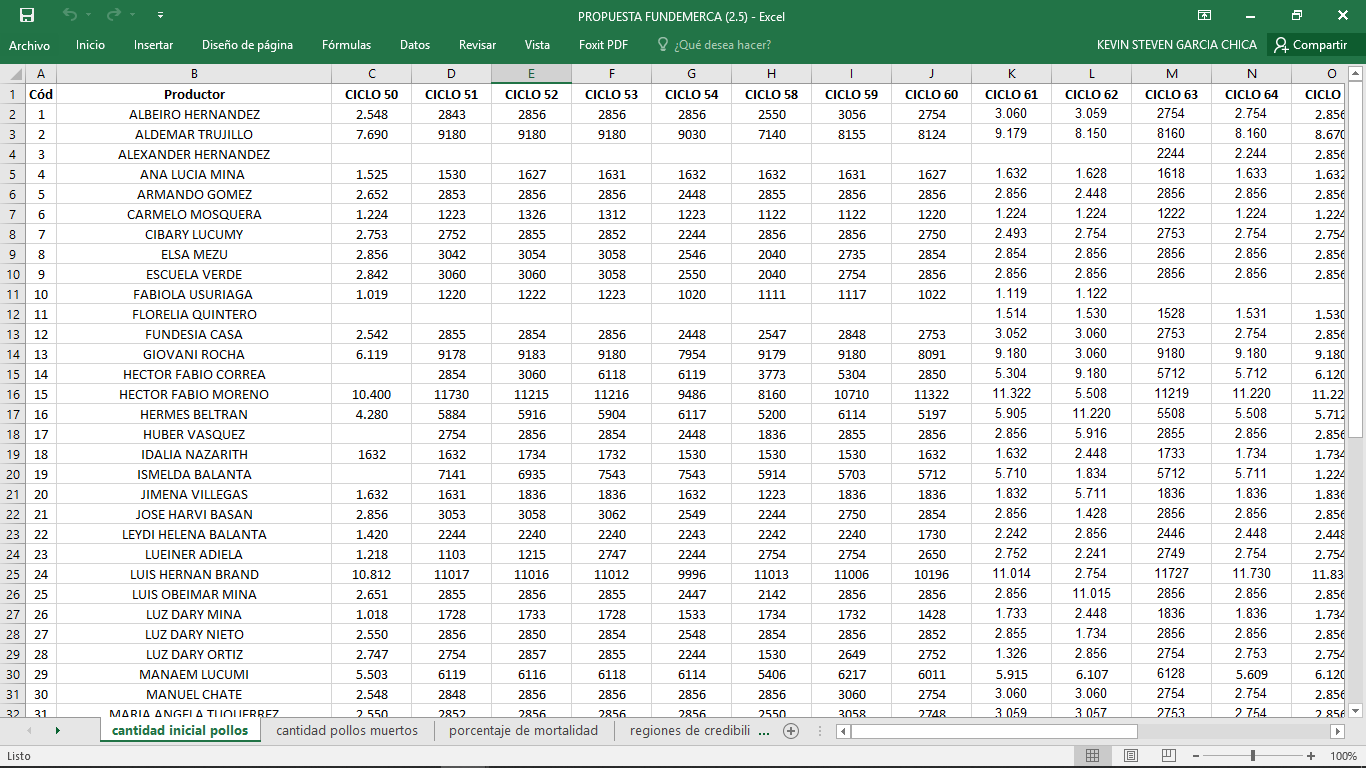
\includegraphics[width=12.3cm]{imagenes/BD.png}
        \label{figura1}
\end{figure}
\end{frame}


\begin{frame}
\frametitle{Metodología y análisis de datos}
\begin{itemize}
\justifying
\item[-]Con la cantidad inicial de pollos y la cantidad de pollos muertos por ciclo para cada productor se automatizó la proporción de pollos muertos.
\item[-]Para cada productor se obtuvo un intervalo para la proporción de pollos muertos con una probabilidad del 95\%, es decir, se entregó dos valores dentro de los cuales se espera que el 95\% de las veces este la proporción real de pollos muertos para ese productor. Esto se realizó para cada ciclo, en otras palabras, cada productor tendrá tantos intervalos como ciclos.
\end{itemize}
\end{frame}

\begin{frame}
\frametitle{Metodología y análisis de datos}
\begin{figure}[!h]
        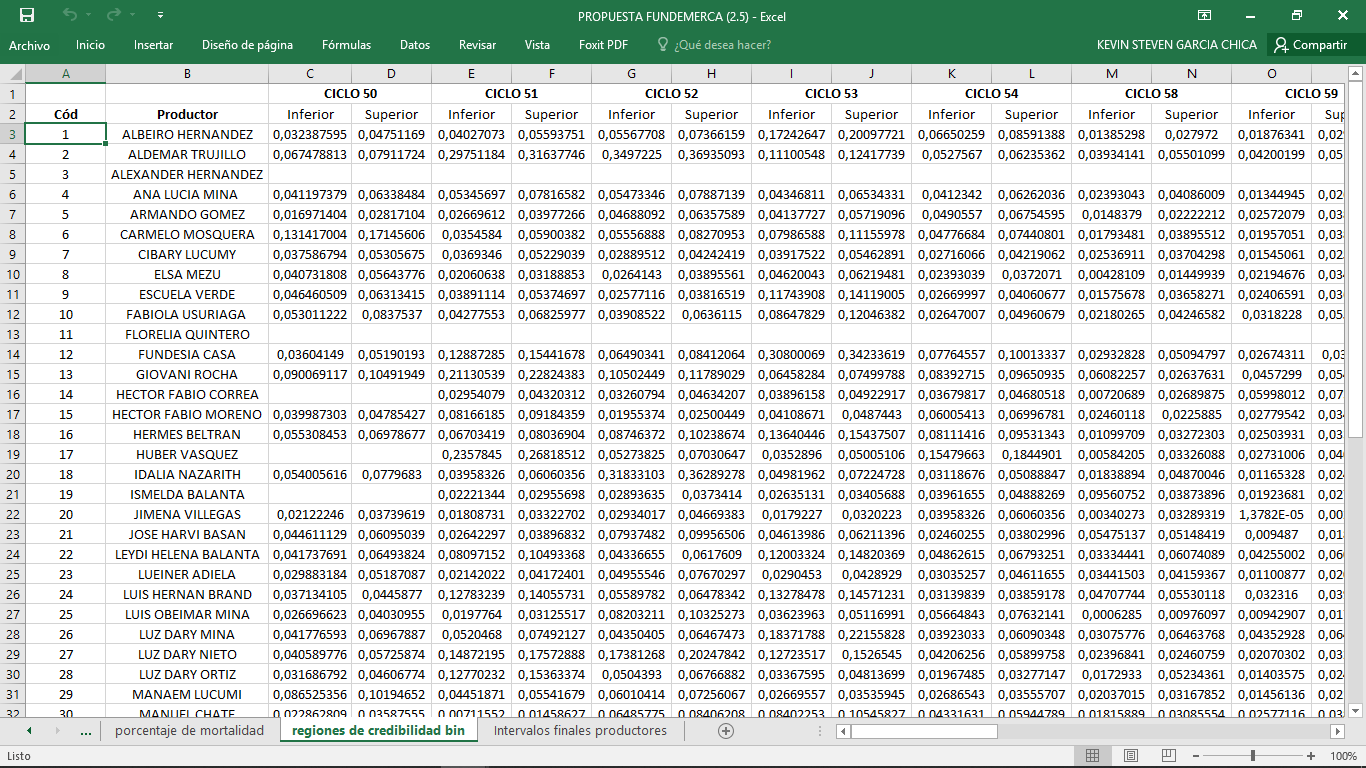
\includegraphics[width=12.3cm]{imagenes/IC.png}
        \label{figura1}
\end{figure}
\end{frame}

\begin{frame}
\frametitle{Metodología y análisis de datos}
\begin{itemize}
\justifying
\item[-]Posteriormente, con todos los intervalos de cada productor, se generaron dos intervalos finales ó generales con los cuales se puede evaluar el desempeño del productor en todos los ciclos. El primero, es el intervalo ``flexible", el cuál se construyo con el mínimo de todos los limites inferiores y el máximo de todos los limites superiores; y el segundo, es el intervalo ``exigente", el cuál se construyó con el máximo de todos los limites inferiores y el mínimo de todos los limites superiores, esto lo que hace es disminuir significativamente la longitud del intervalo. 
\end{itemize}
\end{frame}

\begin{frame}
\frametitle{Metodología y análisis de datos}
\begin{figure}[!h]
        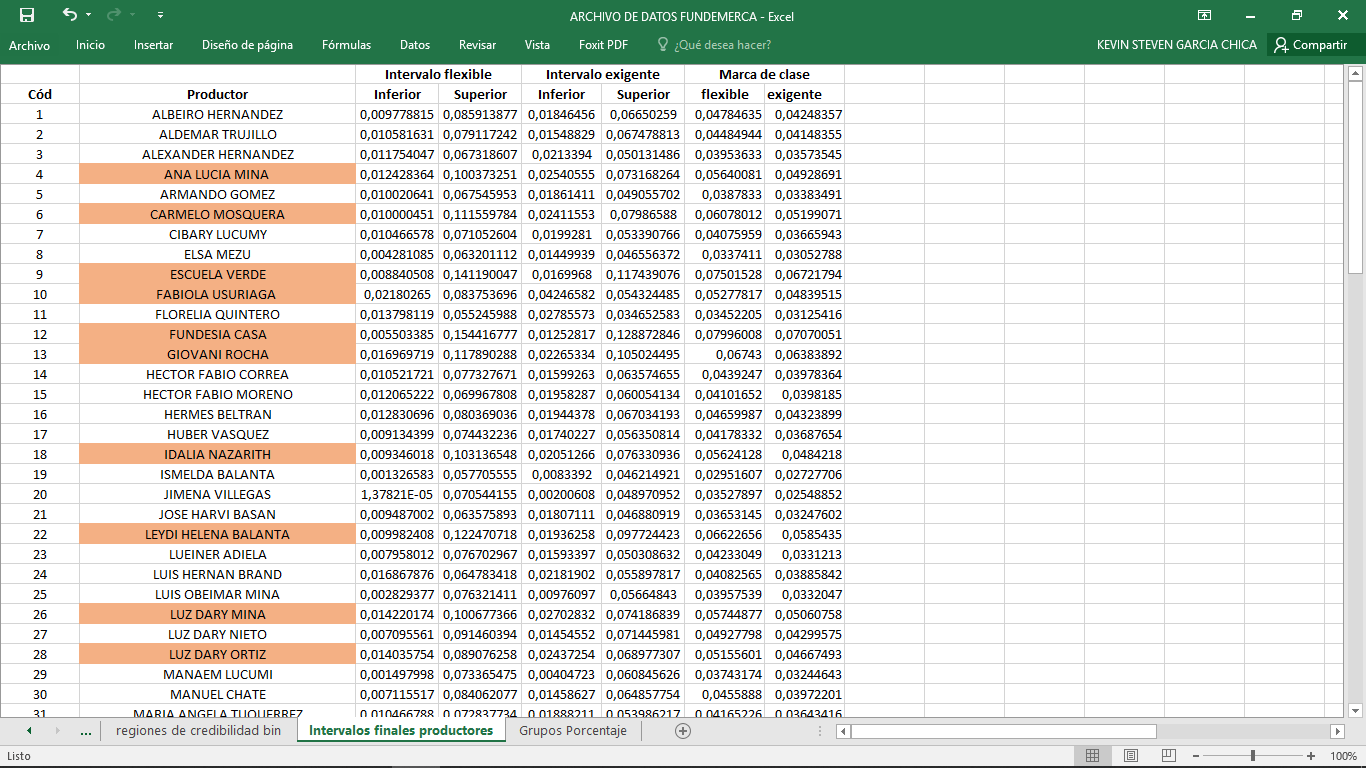
\includegraphics[width=12.3cm]{imagenes/IF.png}
        \label{figura1}
\end{figure}
\end{frame}

\begin{frame}
\frametitle{Metodología y análisis de datos}
\begin{itemize}
\justifying
\item[-]Para la evaluación de los ciclos también se decidió hacer descriptivas, así se puede saber a ciencia cierta si un ciclo tuvo complicaciones y basado en esto no ser injustos con algunos productores.
\item[-]Se realizó un gráfico que nos indica en cada ciclo que proporción de pollos se le murieron a cada productor, por ende, los productores que tienen mas picos en su gráfica indica que la mayoría del tiempo tiene proporciones grandes de muertes
\end{itemize}
\end{frame}

\begin{frame}
\frametitle{Metodología y análisis de datos}
\begin{figure}[!h]
        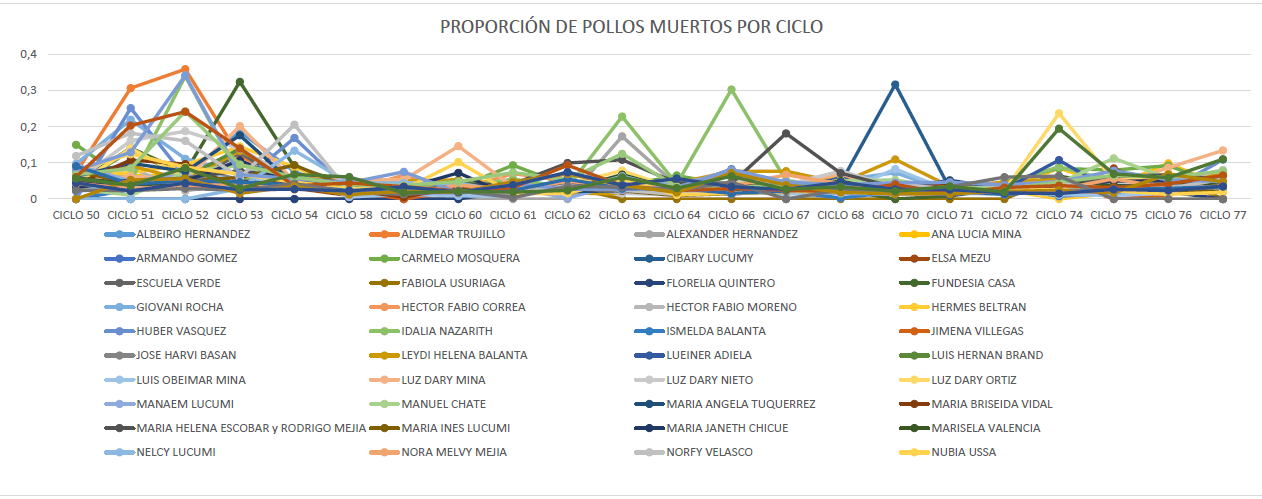
\includegraphics[width=12.3cm]{imagenes/GM.png}
        \label{figura1}
\end{figure}
\end{frame}

\begin{frame}
\frametitle{Metodología y análisis de datos}
\begin{itemize}
\justifying
\item[-]Finalmente, se calculó la probabilidad de que cada productor tenga una proporción de pollos muertos mayor al 5\% en más de la mitad de los ciclos, esta probabilidad sirve para evaluar al productor individualmente.
\item[-]Además, se calculó la probabilidad de que en cada ciclo más de la mitad de los productores tengan una proporción de pollos muertos mayor al 5\%, está probabilidad sirve para evaluar cuales han sido los ciclos más críticos y analizar que ocurrió en ese ciclo en particular.
\end{itemize}
\end{frame}


\begin{frame}
\frametitle{Recomendaciones}
\begin{itemize}
\justifying
\item[-]Se recomienda codificar los productores por orden alfabético para facilitar el manejo de los datos.
\item[-]Cuando un productor no participe en un ciclo se recomienda no eliminarlo, simplemente se deja todo en blanco en dicho ciclo para ese productor, esto facilita que todo el proceso y los datos en general continúen con la misma forma y la misma longitud para evitar confusiones posteriores.
\item[-]Cuando un productor nuevo vaya a ingresar, asignarle el código siguiente, en nuestro caso si entra un nuevo productor se le asignará el código 49, y con este se tienen dos opciones, dejarlo de ultimo siempre sin importar el nombre que tenga, u organizarlo en la base de datos con el orden alfabético pero así mismo se debe editar lo demás (incluirlo en las demás bases) para seguir con la misma organización para todos; la segunda opción sería lo ideal pero demanda mas tiempo.
\end{itemize}
\end{frame}

\begin{frame}
\frametitle{Recomendaciones}
\begin{itemize}
\justifying
\item[-]Hacer un seguimiento anual de los productores para evaluar cuales son los mas eficientes y cuales presentan problemas en la producción (gran porcentaje de pollos muertos).
\item[-]Analizar cada ciclo con el fin de detectar problemas en la producción a tiempo y solucionarlos.
\item[-]Realizar una comparación a lo largo del tiempo de los diferentes años para identificar posibles factores que puedan hacer que un año sea mas productivo que otro.
\end{itemize}
\end{frame}

\begin{frame}
\frametitle{Recomendaciones}
\begin{itemize}
\justifying
\item[-]Suministrar a los productores una bitácora en la cuál puedan llevar control diario sobre los pollos, la cuál debe incluir fecha en la que recibe los pollos, cuantos pollos recibió, cuanto alimento, fecha en la que se muere cada pollo, y otras variables que se consideren importantes para la empresa. Con esto se busca tener un control más estandarizado y mas estricto en cuanto a la cantidad de pollos muertos y las perdidas que estos pueden generar dependiendo de la fecha en que mueran.
\item[-]Definir un plan de muestreo para los productores, con el fin de hacer una visita no anunciada al finalizar cada ciclo. Este plan de muestreo depende de la capacidad en cuanto a logística que tenga la empresa. El objetivo es poder visitar a los 48 productores en todo el año. En la visita se debe revisar la bitácora de los productores y revisar o realizar una especie de auditoria con ellos. 
\end{itemize}
\end{frame}

\begin{frame}
\frametitle{Recomendaciones}
\begin{itemize}
\justifying
\item[-]Establecer un orden de subida de los pollos a los camiones, por ejemplo, agrupar cajas por cantidad de pollos (a un lado del camión poner las cajas que llevan 10 pollos, al otro lado las que llevan 11, en la mitad las que llevan 9, y así sucesivamente), esto con el fin de tener un conteo más exacto de los pollos que salen del productor hacía las bodegas. Esto lo puede realizar el mismo productor en una planilla que se les suministre, en la cuál puedan poner cuantas cajas subieron y con cuantos pollos.
\item[-]Siguiendo la recomendación anterior, se debería estratificar dentro de las bodegas, es decir, dividir la bodega en tres espacios principales (grandes, medianos y pequeños productores) y dentro del mismo estrato o espacio, tener espacios individuales para cada productor. Con esto se logra un control más estricto sobre cada productor y se logra verificar fácilmente la cantidad de pollos que entregó, generando datos más precisos y confiables.
\end{itemize}
\end{frame}
\end{document}